\documentclass[a4paper]{article}
%\documentclass[a4paper,UTF8]{ctexart}

\usepackage{CJKutf8} %设置中文包
%\usepackage{xeCJK} %讓中英文字體分開設置
%\usepackage{CJK} %设置中文包
%\setCJKmainfont{文泉驛等寬正黑} %設定中文為系統上的字型,而英文不去更動,使用原TeX字型
%\XeTeXlinebreaklocale "zh"             %這兩行一定要加,中文才能自動換行
%\XeTeXlinebreakskip = 0pt plus 1pt     %這兩行一定要加,中文才能自動換行
\usepackage[T1]{fontenc} %加這個就可以設定字體 
\usepackage[utf8]{inputenc}
\usepackage{lmodern}
\usepackage{listings}  % 用于代码插入
\usepackage{xcolor} % 用于配色
\usepackage[landscape,  margin=0cm,headsep=0cm]{geometry}
\usepackage{graphicx} %使用图形
\usepackage{amsmath} %使用数学库
\usepackage{amssymb}
\usepackage{mathrsfs}
\usepackage{fullpage}

\usepackage{cmap}
%\usepackage{ccmap}
\usepackage{slashbox}
\usepackage{float}
\usepackage{multicol} %设置多栏
\setlength{\columnseprule}{0.02cm} %设置栏之间的分隔线的宽度,0则不显示分隔线。
\setlength{\columnsep}{0.5cm} %设置栏之间的间隔。

\usepackage{indentfirst}

%\usepackage[dvips]{hyperref}
\usepackage{hyperref}
%\usepackage[pdfencoding=auto,psdextra,bookmark]{hyperref}
%\usepackage[bookmark]{hyperref}
%\usepackage{bookmark}
%\PassOptionsToPackage{unicode}{hyperref}
%\PassOptionsToPackage{naturalnames}{hyperref}
\hypersetup{%
	unicode=true,
	CJKbookmarks=false, 
	bookmarksnumbered=true,
	bookmarksopen=true, 
	bookmarksopenlevel=1, 
	breaklinks=true,
	colorlinks=false, 
	plainpages=false, 
	pdfpagelabels, 
	pdfborder=0 0 0,
	linktocpage=false,
	linkcolor=black, 
	anchorcolor=black, 
	citecolor=black,
    pdfauthor={tiankonguse},
    pdftitle={NENU CS ACM CODE}
}
	%CJKbookmarks=true, %The `CJKbookmarks' option should only be used for    bookmarks *not* in Unicode.`
    %note that option `CJKbookmarks' cannot be used together with option `unicode'.
    %No mechanism is provided to translate non-Unicode bookmarks to Unicode; for portable PDF documents only Unicode encoding should be used.
\usepackage{fancyhdr}
\pagestyle{fancy}
\fancypagestyle{plain}{
    \pagestyle{fancy}
}



%对齐方式
%左对齐 \begin{flushleft}...\end{flushleft}搜索
%居中 \begin{center}...\end{center}
%右对齐 \begin{flushright}...\end{flushright}
%linespread 设置行距

%打印公式符号
% 打印 % => \%
% 打印 ^ => \^{}
% 打印 _ => \_
%     + => \#
%     $ => \$
%     { => \{
%     } => \}
%     ~ => \~ ,推荐 $\sim$
%     & => \&
%     | => $|$
%     < => $<$
%     > => $>$
%     * => $*$
%


%页眉和页脚的左部,中部,右部
\lhead{\thepage}
\chead{\textit{NENU CS ACM CODE}}
\rhead{\thepage}
%\lfoot{\thepage}
\lfoot{}
\cfoot{make by \href{http://tiankonguse.com/}{tiankonguse} \& powered      by nenu CS acmer and vici \& v0.6}
\rfoot{\thepage}
\renewcommand{\headrulewidth}{0.01cm}
\renewcommand{\footrulewidth}{0cm}

%定义一个名为 darkgreen 的颜色
\xdefinecolor{darkgreen}{rgb}{0,0.35,0}

%设置插入的代码的样式
\lstset{
    tabsize=4,%tab键用四个空格替换
    basicstyle=\ttfamily\scriptsize,
    extendedchars=false, %解决代码跨页时,章节标题,页眉等汉字不显示的问题
  	escapechar=`, %中文添加`后,可以避免注释中如果含有中文则顺序错乱
    breaklines=true,      %让LaTeX自动将长的代码行换行排版
    breakatwhitespace=false,
    language=C++,   %让LaTeX排版时将C++键字突出显示
    keywordstyle=\textbf, %for printing
    morekeywords={bool,__int64},
    keywordstyle=\color{blue!90},%关键词的颜色
    commentstyle=\color{darkgreen!85},%注释的颜色
    rulesepcolor=\color{red!20!green!20!blue!20},
    basicstyle=\footnotesize\ttfamily, %for paste
    columns=flexible,
%	showspaces=false,
%	showtabs=false,
%	numbers=left, 
%	numberstyle=\tiny,
%	frame=shadowbox, 
%	rulesepcolor=\color{red!20!green!20!blue!20},
    xrightmargin=0.5em %右边距
}

\title{ACM CODE}
\author{\href{http://tiankonguse.com/}{tiankonguse}}
\date{\today}

\begin{document}
%使用CJK中文 ,仿宋格式
\begin{CJK*}{UTF8}{gbsn}
%\begin{CJK*}{UTF8}{song}

%首页是封面,所以应该显示一栏
\begin{onecolumn}

\maketitle

%插入图片
\centering{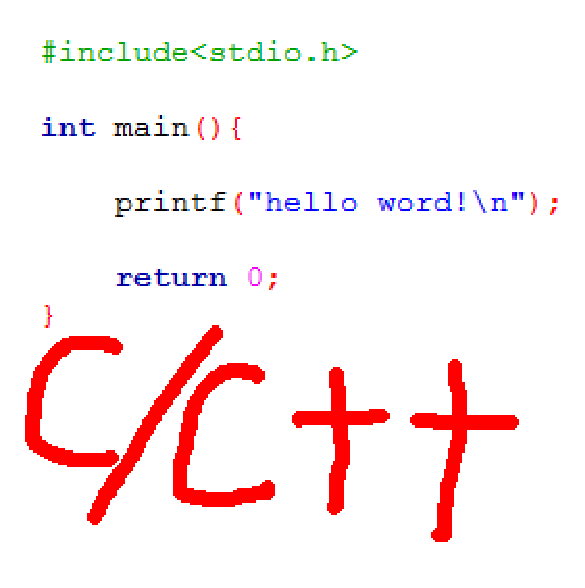
\includegraphics[width=10cm]{front.eps}}

\end{onecolumn}

%新的一页
\clearpage

\center{this is a blank page.}

%新的一页
\clearpage

%设置多栏
\begin{multicols}{3}

%设置目录的名字
\renewcommand{\contentsname}{目录}

%生成目录
\tableofcontents

\clearpage 

%全部左对齐
\begin{flushleft} 

% 
% section{一级目录}
%
% 
%subsection{二级目录}
%
%\begin{lstlisting}[language={代码语言}]
% 插入代码
%  //`代码注释全部用这个引起来,防止因为中文引起顺序错乱`
%\end{lstlisting}
%
%lstinputlisting 可以程序导入文件
%
\section{Base}
\subsection{头文件}
%\cppcode{header.cpp}
\lstinputlisting[language={C++}]{source/base/header.cpp}

\subsection{文件结束符}
\lstinputlisting[language={C++}]{source/base/file_endsign.cpp}

\subsection{codeblock配置终端}
\lstinputlisting[language={C++}]{source/base/codeblock_setting.cpp}

\subsection{codeblock快捷键}
\lstinputlisting[language={C++}]{source/base/codeblock_shortcuts.cpp}

\subsection{通用long long}
\lstinputlisting[language={C++}]{source/base/normal_long_long.cpp}

\subsection{设置栈的大小}
\lstinputlisting[language={C++}]{source/base/set_stack_size.cpp}

\subsection{Faster\_IO(G++ is better)}
\lstinputlisting[language={C++}]{source/base/faster_io.cpp}


\subsection{Notes}
\lstinputlisting[language={C++}]{source/base/notes.cpp}



\clearpage 

\section{数据结构}

\subsection{数的范围}
\lstinputlisting[language={C++}]{source/dataStructure/number_range.cpp}

\subsection{素数专题}
素数定理:pi(x)/x*ln(x)=1,pi(x)表示小于x的素数的个数
孪生素数猜想:存在无穷个p,p+2的素数对
PS:陈景润证明的存在无穷个素数p,p+2至多有两个素数因子,及传说当中的"1+2"问题
哥德巴赫猜想:每个大于2的偶数是两个素数的和
$n^2+1$猜想:存在无穷个$n^2+1$这样形式的素数
埃拉托斯尼斯筛法:正整数n是素数,当且仅当它不能被任何小于n的平方根的素数整除。
有时候素数的范围很大,不能把所有的素数表打出来,就要只存部分素数。 
如果求区间的素数,就对区间进行筛法



\subsubsection{素数定理}
对正实数x,定义π(x)为素数计数函数,亦即不大于x的素数个数。
简单表达式:$\pi(x)\approx\frac{x}{\ln\,x}$,其中ln x为x的自然对数。
精确表达式:$\pi(x)={\rm Li} (x) + O \left(x e^{-\frac{1}{15}\sqrt{\ln\,x}}\right)$,其中 ${\rm Li} (x) = \int_2^x \frac{dt}{\ln\,t}$

\subsubsection{素数表基本晒法}
\lstinputlisting[language={C++}]{source/dataStructure/sieve_base_prime.cpp}

\subsubsection{压位筛素数}
\lstinputlisting[language={C++}]{source/dataStructure/sieve_bit_prime.cpp}

\subsubsection{sieve}
\lstinputlisting[language={C++}]{source/dataStructure/sieve_mark_prime.cpp}

\subsubsection{小舟学长的筛法}
\lstinputlisting[language={C++}]{source/dataStructure/sieve_vici_prime.cpp}

\subsubsection{区间素数}
\lstinputlisting[language={C++}]{source/dataStructure/sieve_range_prime.cpp}

\subsubsection{sieve 100000 primes \texorpdfstring{$>$} 1e12}
\lstinputlisting[language={C++}]{source/dataStructure/sieve_large_prime.cpp}

\subsubsection{反素数}
\lstinputlisting[language={C++}]{source/dataStructure/anti_prime.cpp}



\subsection{大素数}
\lstinputlisting[language={C++}]{source/dataStructure/huge_prime.cpp}



\subsubsection{检验n是不是合数}
\lstinputlisting[language={C++}]{source/dataStructure/huge_prime_check_composite.cpp}



\subsubsection{大素数测试}
\lstinputlisting[language={C++}]{source/dataStructure/huge_prime_test.cpp}

\subsubsection{pollard\_rho分解}
\lstinputlisting[language={C++}]{source/dataStructure/pollard_rho.cpp}


\subsubsection{质因数分解N }
\lstinputlisting[language={C++}]{source/dataStructure/huge_prime_find.cpp}

\subsection{梅森素数}
m是一个素数,$M=2^m-1$也是一个素数,则M是梅森素数。
使用大素数测试得到森素数。

\subsubsection{Lucas-Lehmer判定法}
\lstinputlisting[language={C++}]{source/dataStructure/lucas_lehmer.cpp}

\subsection{同余}
两个整数a,b,若它们除以正整数m所得的余数相等,则称a,b对于模m同余
记作$a \equiv b \pmod{m}$


\subsection{费马大定理}
当整数n>2时,关于x, y, z的不定方程 $x^n + y^n =z^n$.的整数解都是平凡解
当n是偶数时:$(0,\pm m,\pm m)$或$(\pm m,0,\pm m)$
当n是奇数时:$(0,m,m), (m,0,m)$或$(m,-m,0)$



\subsection{费马小定理}
如果p是素数,则$a^{p-1} \equiv  1 \pmod{p}$对所有整数a都成立


\subsection{欧拉函数}

\subsubsection{欧拉定理}
$a^{\varphi(n)} \equiv 1 \pmod n, \gcd(a,n)=1$

\subsubsection{一些结论}
a为N的质因数
若 (N/a)\%a == 0 则有 E(N) = E(N/a)*a.
若 (N/a)\%a !=0则有 E(N) = E(N/a)*(a-1)
一个数的所有质因子之和 F(n)*n/2.


\subsubsection{原根}
在gcd(a,m)=1时,定义a对模m的指数$Ord_m(a)$为使$a^d \equiv 1 \pmod{m}$成立的最小的正整数d。
由前知$Ord_m(a) $一定小于等于$  \phi (m)$,若$Ord_m (a) = \phi (m)$,则称a是模m的原根。
设m是正整数,a是整数,若a模m的阶等于φ(m),则称a为模m的一个原根

\lstinputlisting[language={C++}]{source/dataStructure/primitive_root.cpp}


\subsubsection{与n互素的数的和}
$$\sum_{1 \le k \le n}^{(k,n)=1} k = \frac{1}{2} n \varphi(n)$$


\subsubsection{第n个与m互质的数}
如果求与m互质的第n个数,可以先把小于m的互质的数错在ans中(筛法求)
(从1开始存,最后一个存在0中),然后大于m的互质的数都是小于m的互质的数加上若干个m得到的。

\lstinputlisting[language={C++}]{source/dataStructure/nth_prime.cpp}

\subsection{sieve phi}
\lstinputlisting[language={C++}]{source/dataStructure/sieve_phi.cpp}

\subsubsection{打表欧拉函数}
\lstinputlisting[language={C++}]{source/dataStructure/phi_tanle.cpp}


\subsubsection{单独求欧拉函数(公式)}
\lstinputlisting[language={C++}]{source/dataStructure/phi_single.cpp}

\subsubsection{容斥求小于a的与n互质的个数}
\lstinputlisting[language={C++}]{source/dataStructure/phi_kth.cpp}

\subsection{随机数}
\lstinputlisting[language={C++}]{source/dataStructure/rand_number.cpp}

\subsection{二分}

\subsubsection{最大值最小化问题}
m个正整数的序列划分成m个子连续序列,每个子序列的个数字之和为S, 使所有S中的最大S最小。\\

\subsubsection{数轴上点到点的距离和}
点的中位数就是答案\\
如果点有奇数个,答案唯一。\\
如果点有偶数个,答案是个区间\\

\subsubsection{数轴上点到点的距离平方和}
列出方程后,可以证明是个凸函数。\\
于是这个可以使用三分做。\\
猜想可能还是中位数。\\

\subsubsection{坐标系上点到点的曼哈顿距离和}
此时,x轴与y轴没有关系了,找到x轴的中位数与y轴的中位数即可。\\

\subsubsection{...到点的距离平方和}
这个经过列出等式后,可以发现,每一维是相互独立的。\\
而转化成了在数轴上的距离平方和问题了。\\

\subsubsection{...到点的距离和}
这个需要偏导数理论。\\
写出偏导数后发现当其他维数固定时,这个维数还是相互独立的。\\
但是不使用偏导数时,我们只需使用变步长寻找即可。\\
例如:\\
1. 取步长为step,起点为(x0,y0)\\
2. 我们找到上下左右的四个点的值,如果有比(x0,y0)更优的值,则更新(x0,y0)。\\
3. 循环执行步骤2,直到(x0,y0)就是最优值。\\
4. 此时,步长变为原来的0.5倍,继续执行步骤2.直到step达到一定的精度。\\

\subsubsection{...到直线的距离和}
思考中\\


\subsubsection{...到直线的距离平方和}
思考中\\



\subsection{贪心}

\subsubsection{区间选点问题}
取尽量少的点,使每个区间内都至少有一个点。\\

\subsubsection{区间覆盖问题}
数轴上有若干区间,选尽量少的区间,覆盖指定区间。\\


\subsection{GCD}


\subsubsection{GCD(无递归)}
\lstinputlisting[language={C++}]{source/dataStructure/gcd_noRecursion.cpp}



\subsubsection{GCD(递归)}
\lstinputlisting[language={C++}]{source/dataStructure/gcd_recursion.cpp}

\subsubsection{快速GCD}
\lstinputlisting[language={C++}]{source/dataStructure/gcd_fast.cpp}

\subsubsection{fgcd}
\lstinputlisting[language={C++}]{source/dataStructure/gcd_float.cpp}


\subsubsection{GCD结论}
有俩个数p,q,且gcd(q,p)=1,则最大无法表示成px+qy(x>=0,y>=0)的数是pq-q-p.\\

\subsubsection{区间内与n的gcd不小于m的个数 }
输入m, n,求1~n之间中gcd(x, n) >=m 的x个数。\\
找出N的所有大于等于M的因子(x1,x2,x3.....xi),然后设k=N/xi;\\
下面只需找出小于k且与k互质的数。\\
因为:设y与k互质且小于k,那么gcd(y*xi,k*xi)=xi;(xi为N的因子,且xi大于等于M)。\\

\subsubsection{LCM}
\lstinputlisting[language={C++}]{source/dataStructure/lcm.cpp}


\subsection{扩展GCD}
\lstinputlisting[language={C++}]{source/dataStructure/kgcd.cpp}


\subsubsection{解不定方程ax + by =n}
(1)计算gcd(a,b)\\
若d=gcd(a,b)不能整除n,则方程无整数解;\\
否则,在方程的两边同除以gcd(a,b),得到新的不定方程a'x+b'y=n',此时gcd(a' ,b')=1。\\
(2) 求出不定方程a'x+b'y=1的一组整数解x0,y0,则n'x0,n'y0是方程a'x+b'y=n'的一组整数解。(用扩展欧几里得求x0,y0)\\
(3)可得方程a'x+b'y=n'的所有整数解为:x=n'x+b't;y=n'y0-a't(t为整数)\\
这就是方程ax+by=n的所有整数解\\
x,y是通解\\
x=n/d*x0+b/d*t\\
y=n/d*y0-a/d*t\\
(t是整数) \\

\subsubsection{求(a/b)\% c(乘法逆元)}
\lstinputlisting[language={C++}]{source/dataStructure/inverse.cpp}

\subsubsection{模线性方程 a*x=b(mod n)}
\lstinputlisting[language={C++}]{source/dataStructure/linear_equations.cpp}


\subsection{因子}
\subsubsection{所有数的因子的个数 O(n*log(n))}
\lstinputlisting[language={C++}]{source/dataStructure/number_of_factor_all_number.cpp}


\subsubsection{所有数的因子的个数 O(n)}
\lstinputlisting[language={C++}]{source/dataStructure/number_of_factor_all_number_line.cpp}


\subsubsection{一个数的因子的个数}
\lstinputlisting[language={C++}]{source/dataStructure/number_of_factor_a_number.cpp}

\subsubsection{一个数的所有因子之和}
\lstinputlisting[language={C++}]{source/dataStructure/sum_of_factor_a_number.cpp}

\subsection{MOD}
\lstinputlisting[language={C++}]{source/dataStructure/mode.cpp}
 
\subsubsection{(a*b)\%c  muti\_mod1}
\lstinputlisting[language={C++}]{source/dataStructure/muti_mod.cpp}

\subsubsection{(a*b)\%c  muti\_mod2}
\lstinputlisting[language={C++}]{source/dataStructure/muti_mod2.cpp}

\subsubsection{\texorpdfstring{$a^b$}.\%c pow\_mod1}
\lstinputlisting[language={C++}]{source/dataStructure/pow_mod1.cpp}

\subsubsection{powMod}
\lstinputlisting[language={C++}]{source/dataStructure/pow_mod2.cpp}

\subsubsection{powMod\_plus}
\lstinputlisting[language={C++}]{source/dataStructure/pow_mod_plus.cpp}

\subsubsection{\texorpdfstring{$x^n$}.\% c 非递归}
\lstinputlisting[language={C++}]{source/dataStructure/pow_mod_nonrecursive.cpp}

\subsubsection{求\texorpdfstring{$a^b$}.\% c binary}
\lstinputlisting[language={C++}]{source/dataStructure/pow_mod_binary.cpp}

\subsubsection{Lucas定理 求C(n+m,n)\%p}
\lstinputlisting[language={C++}]{source/dataStructure/lucas.cpp}

\subsubsection{C(n,m)\%mod (div)}
\lstinputlisting[language={C++}]{source/dataStructure/lucas_div.cpp}

\subsubsection{C(n,m)\%mod (inv)}
\lstinputlisting[language={C++}]{source/dataStructure/lucas_inv.cpp}

\subsubsection{迭代幂}
\lstinputlisting[language={C++}]{source/dataStructure/power_iterative.cpp}

\subsubsection{\texorpdfstring{$A^x$}.\% C==b}
\lstinputlisting[language={C++}]{source/dataStructure/baby_step.cpp}

\subsection{汉若塔问题}
\lstinputlisting[language={C++}]{source/dataStructure/tower_of_hanoi.cpp}


\subsection{字母大小写转换 位操作}
\begin{lstlisting}[language={c++}]
'A'^'a' = 32; 
\end{lstlisting}

$$$$
\subsection{二项式展开}
$$(a+b)^n = \sum_{k=0}^n C_n^ka^{n-k}b^k$$\\


\subsection{阶乘}

\subsubsection{阶乘的位数(仅有位数)}
\lstinputlisting[language={C++}]{source/dataStructure/factorial_bits.cpp}


\subsubsection{阶乘0的个数}
\lstinputlisting[language={C++}]{source/dataStructure/factorial_zero_number.cpp}


\subsubsection{阶乘最后非0位}
\lstinputlisting[language={C++}]{source/dataStructure/factorial_last_nozero.cpp}


\subsubsection{阶乘分解}
\lstinputlisting[language={C++}]{source/dataStructure/factorial_number_of_factor.cpp}


\subsubsection{阶乘的位数(求各位数字)}
高精度乘法\\


\subsubsection{阶乘素数因子个数}
\lstinputlisting[language={C++}]{source/dataStructure/factorial_number_of_factor2.cpp}

\subsubsection{快速乘方\texorpdfstring{$a^k$}.}
\lstinputlisting[language={C++}]{source/dataStructure/pow_fast.cpp}


\subsubsection{\texorpdfstring{$A^B$ }.次方的首位数字}
\lstinputlisting[language={C++}]{source/dataStructure/pow_first.cpp}



\subsection{二进制中一的个数}

\subsubsection{自底向上分治法O(5)}
\lstinputlisting[language={C++}]{source/dataStructure/bit_of_number_divide.cpp}


\subsubsection{复杂度为1的个数}
\lstinputlisting[language={C++}]{source/dataStructure/bit_of_number_xor.cpp}


\subsubsection{朴素的算法O(32)}
\lstinputlisting[language={C++}]{source/dataStructure/bit_of_number_line.cpp}

\subsection{树根}
\begin{lstlisting}
root(a+b)=root(root(a) + root(b)) 
root(a*b)=root(root(a) * root(b)) 
root(a)=root(root(a/10) + a\%10)
\end{lstlisting}

\subsubsection{n的树根 模拟}
\lstinputlisting[language={C++}]{source/dataStructure/root_number_simulation.cpp}

\subsubsection{n的树根 找规律}
\lstinputlisting[language={C++}]{source/dataStructure/root_number_pattern.cpp}

\subsubsection{n的树根 高精度}
\lstinputlisting[language={C++}]{source/dataStructure/root_number_precision.cpp}

\subsubsection{\texorpdfstring{$n^n$}.的树根 找规律}
\lstinputlisting[language={C++}]{source/dataStructure/pow_root_pattern.cpp}

\subsubsection{\texorpdfstring{$n^n$}.的树根 模拟}
\lstinputlisting[language={C++}]{source/dataStructure/pow_root_simulation.cpp}

\subsubsection{\texorpdfstring{$a^b$}.的树根 模拟}
\lstinputlisting[language={C++}]{source/dataStructure/pow_root_simulation2.cpp}

\subsubsection{\texorpdfstring{$a^b$}.的树根 二进制法}
\lstinputlisting[language={C++}]{source/dataStructure/pow_root_binary.cpp}

\subsection{公式}

\subsubsection{三角公式}
Atan2(x,y):结果是以弧度表示(-PI,PI)\\
Atan2(0,-1)=PI\\

\subsubsection{数学公式}
sum(k)=(n+1)*n/2\\
sum(k\^{}2)=n (n+1)(2n+1)/6\\
sum(k\^{}3)=(n (n+1)/2)\^{}2\\
sum(k\^{}4)=n (n+1) (2n+1) (3n\^{}2+3n-1)/30\\
sum(k\^{}5)= n\^{}2 (n+1)\^{}2 (2n\^{}2+2n-1)/12\\
sum(k(k+1))=n(n+1)(n+2)/3\\
sum(k(k+1)(k+2))=n(n+1)(n+2)(n+3)/4\\
sum(k(k+1)(k+2)(k+3))=\\
n(n+1)(n+2)(n+3)(n+4)/5\\

\subsubsection{精度公式}
\lstinputlisting[language={C++}]{source/dataStructure/high_double.cpp}

\subsubsection{对数公式}
\begin{lstlisting}
`$log_a^n + log_a^m = log_{a}^{nm} $`
`$k*log_a^n = log_{a}^{n^k}$ `
`换底公式: $log_a^n/log_b^n=log_b^a $`
\end{lstlisting}

\subsubsection{复杂度公式}
\begin{lstlisting}
`递归式T(n) = aT(n/b) + f(n)`
`递归树结果`
`T(n) = f(n)+af(n/b)+a\^{}2f(n/b\^{}2)+…a\^{}Lf(n/b\^{}L)其中$L=log_bn $`
\end{lstlisting}

\subsection{微积分}

\subsubsection{曲线长度}
\begin{lstlisting}
`在y=f(x)的任意点(x,y)附近去一段小曲线,看成线段,其长度:`
Ds = sqrt(dx\^{}2 + dy\^{}2) 
= dx sqrt(1 + (dy/dx)\^{}2 )
= sqrt(1 + f'(x)\^{}2 ) dx
`所以:`s = sqrt(1 + f'(x)\^2{}) [x2,x1]
\end{lstlisting}

\subsubsection{二次函数}
\begin{lstlisting}
`对于抛物线一般式:`y=ax^2 + bx + c, y’ = 2ax + b
ds = sqrt(1 + f’(x)^2)
 = sqrt(1 + (2ax + b)^2)dx 
 = 1/2a * sqrt(1 + (2ax+b)^2) d(2ax+b)
 = 1/2a * sqrt(1 + t^2) dt
 = 1/4a * (t * sqrt(1 + t^2) + ln(t + sqrt(1 + t^2))) [x2,x1]
\end{lstlisting}

\subsection{约瑟夫环的数学方法}
\lstinputlisting[language={C++}]{source/dataStructure/joseph_math.cpp}

\subsubsection{pick定理}
如果顶点都为整数坐标点,面积=边点/2+内点-1\\

\subsection{catalan数}
卡特兰数前几项
1, 1, 2, 5, 14, 42, 132, 429, 1430, 4862, 16796, 58786, 208012, 742900, 2674440, 9694845, 35357670, 129644790, 477638700, 1767263190, 6564120420, 24466267020, 91482563640, 343059613650, 1289904147324 

\subsubsection{等价公式}
\begin{lstlisting}
h(n)= h(0)*h(n-1)+h(1)*h(n-2) + ... + h(n-1)h(0) (n>=2)
h(n)=h(n-1)*(4*n-2)/(n+1)
h(n)=C(2n,n)/(n+1) (n=1,2,3,...)
h(n)=c(2n,n)-c(2n,n+1)(n=1,2,3,...)
H(n+1) = 2(2n+1)/(n+2) * H(n)
H(n+1)=sum(H(i)*H(n-i)) (0<=i<=n)
H(n) = sum( C(n,i) * C(n,i) ) /(n+1) (0<=i<=n)
H(n) = 4^n/(n^1.5 * sqrt(pi))
\end{lstlisting}

\subsubsection{应用}
\begin{lstlisting}
`1.n个数的不同出栈序列`
`2.N个+1和n个-1构成2n项a1a2...an,其部分和满足a1+a2+a3+...+an>=0,0<=k<=2n。满足这个序列的个数等于第n个catakan数。`
`3.括号匹配的合法个数`
`4.连乘的选择个数`
`5.n个节点的二叉树的树的形态的个数。`
`6.n个非叶子节点的满二叉树的形态数。`
`7.n*n的矩阵中,从右下角到左上角的走法。`
`8.凸n+2边形进行三角分割数。`
`9.n层的阶梯切割为n个矩阵的切割法数。`
`10.在一个2*n的格子中填入1到2n这些数字,使每个格子内的数值都比其右边和上边的所有数值都小的情况数。`
\end{lstlisting}

\subsection{随机函数}
\lstinputlisting[language={C++}]{source/dataStructure/rands.cpp}

\subsection{积性函数}
对于正整数n的一个函数f(n),当中f(1)=1且当a,b互质时,f(a,b)=f(a) * f(b);\\
若某函数f(n)富符合f(1)=1,且就算a,b不互质,f(a,b)=f(a) * f(b),则称它为完全积性函数。\\

积性函数有:\\
欧拉函数:计算与n互质的小于n的正整数的个数\\
莫比乌斯函数:关于非平方数的质数因子的数目\\
gcd(n,k):最大公因子,k固定\\
d(n):n的正因子数目,n的所有正因子之和\\

\subsection{三分算法}
\lstinputlisting[language={C++}]{source/dataStructure/third_div.cpp}

\subsection{位操作}

\subsubsection{与操作}
i. 用以取出一个数的某些二进制位\\
ii. 取出一个数二进制中的最后一个 1:x\&-x

\subsubsection{或操作}
用以将一个数的某些位设为1\\

\subsubsection{非操作}
用以间接构造一些数:$\sim$0u=4294967295=$23^2$-1\\
INI\_MAX = ($\sim$0u)$>$$>$1\\


\subsubsection{异或操作}
i. 不使用中间变量交换两个数:a=a\^{}b;b=a\^{}b;a=a\^{}b; \\
ii. 将一个数的某些位取反\\



\subsection{矩阵}
\lstinputlisting[language={C++}]{source/dataStructure/matrix.cpp}


\subsubsection{矩阵相乘}
\lstinputlisting[language={C++}]{source/dataStructure/matrix_mul.cpp}

\subsubsection{矩阵幂乘}
\lstinputlisting[language={C++}]{source/dataStructure/matrix_pow.cpp}

\subsubsection{判断A*B==C 随机算法}
\lstinputlisting[language={C++}]{source/dataStructure/matrix_eq_rand.cpp}

\subsubsection{判断A*B==C 伪随机算法}
A*B的复杂度是O($n^3$),A是一维的话,复杂度就是O($n^2$)了。\\
所以A*B == C 可以近似的转化为1 * A * B == 1 * C\\
1是一维的向量。\\

\subsubsection{矩阵幂相加}
给定矩阵A,求$A + A^2 + A^3 + ... + A^k$的结果(两个矩阵相加就是对应位置分别相加)。输出的数据mod m。$k<=10^9$。\\
这道题两次二分,相当经典。\\
首先我们知道,$A^i$可以二分求出。\\
然后我们需要对整个题目的数据规模k进行二分。\\
比如,当k=6时,有:$A + A^2 + A^3 + A^4 + A^5 + A^6 =(A + A^2 + A^3) + A^3*(A + A^2 + A^3)$\\
应用这个式子后,规模k减小了一半。\\
我们二分求出$A^3$后再递归地计算$A + A^2 + A^3$,即可得到原问题的答案。\\

\subsection{构造矩阵}

\subsubsection{求第 n 个 Fibonacci 数 mod p}
给定 n 和 p,求第 n 个 Fibonacci 数 mod p 的值,n 不超过 2\^{}31\\
现在我们需要构造一个 2 x 2 的矩阵,使得它乘以(a,b)得到的结果是(b,a+b)。\\
每多乘一次这个矩阵,这两个数就会多迭代一次。\\
那么,我们把这个 2 x 2 的矩阵自乘 n 次,再乘以(0,1)就可以得到第 n 个 Fibonacci 数了。\\
不用多想,这个 2 x 2 的矩阵很容易构造出来:\\
\begin{math}
\begin{pmatrix}
	0 & 1  \\
    1 & 1
\end{pmatrix}
\cdot
\begin{pmatrix}
	a  \\
    b 
\end{pmatrix}
=
\begin{pmatrix}
	b  \\
    a+b 
\end{pmatrix}
\end{math}

\subsubsection{A 走 k 步到 B 的方案数}
给定一个有向图,问从 A 点恰好走 k 步(允许重复经过边)到达 B 点的方案数 mod p 的值\\
把给定的图转为邻接矩阵,即 A(i,j)=1 当且仅当存在一条边 i->j。\\
令 C=A*A,那么C(i,j)=ΣA(i,k)*A(k,j),实际上就等于从点 i 到点 j 恰好经过 2 条边的路径数(枚举 k 为中转点)。\\
类似地,C*A 的第 i 行第 j 列就表示从 i 到 j 经过 3 条边的路径数。\\
同理,如果要求经过 k 步的路径数,我们只需要二分求出 A\^{}k 即可。\\

\subsubsection{用1x2填充MxN的矩阵}
用 1 x 2 的多米诺骨牌填满 M x N 的矩形有多少种方案,M$<$=5,N$<$2\^{}31,输出答案 mod p 的结果\\

\subsection{高斯消元法}
\lstinputlisting[language={C++}]{source/dataStructure/gauss.cpp}

\subsection{母函数}
\subsubsection{母函数(整数拆分)}
\lstinputlisting[language={C++}]{source/dataStructure/generating_function_integer_split.cpp}

\subsubsection{指数型母函数}
\lstinputlisting[language={C++}]{source/dataStructure/generating_function_index.cpp}

\subsection{约瑟夫问题}
\lstinputlisting[language={C++}]{source/dataStructure/joseph.cpp}

\subsection{汉诺塔升级版}
\lstinputlisting[language={C++}]{source/dataStructure/tower_of_hanoi_upgrade.cpp}

\subsection{快速排序}
\lstinputlisting[language={C++}]{source/dataStructure/quick_sort.cpp}

\subsection{堆}
\lstinputlisting[language={C++}]{source/dataStructure/heap.cpp}

\subsection{最大堆}
\lstinputlisting[language={C++}]{source/dataStructure/heap_max.cpp}

\subsection{堆排序}
\lstinputlisting[language={C++}]{source/dataStructure/heap_sort.cpp}

\subsection{归并排序求逆序数}
\lstinputlisting[language={C++}]{source/dataStructure/reverse_number_by_merger_sort.cpp}

\subsection{取第 k 个元素}
\lstinputlisting[language={C++}]{source/dataStructure/number_kth.cpp}

\subsection{Pell 方程}
\lstinputlisting[language={C++}]{source/dataStructure/pell.cpp}

\subsection{区间合并}
可以先对区间排序;然后简单合并即可\\

\subsection{星期几}
\lstinputlisting[language={C++}]{source/dataStructure/week.cpp}

\subsection{线段树}

\subsubsection{单点更新}
\lstinputlisting[language={C++}]{source/dataStructure/segment_tree_single_point.cpp}

\subsubsection{成段更新}
\lstinputlisting[language={C++}]{source/dataStructure/segment_tree_segments.cpp}


\subsubsection{应用}
\lstinputlisting[language={C++}]{source/dataStructure/segment_tree_application.cpp}

\subsection{树套树}
\subsubsection{线段树套平衡树}
\lstinputlisting[language={C++}]{source/dataStructure/segment_tree_cover_balanced_tree.cpp}

\subsubsection{划分树}
\lstinputlisting[language={C++}]{source/dataStructure/partition_tree.cpp}

\subsection{左偏树}
\lstinputlisting[language={C++}]{source/dataStructure/left_side_tree.cpp}

\subsection{DLX}
\lstinputlisting[language={C++}]{source/dataStructure/dlx.cpp}

\subsection{AC 自动机}
\lstinputlisting[language={C++}]{source/dataStructure/AC_automaton.cpp}

\subsubsection{传统字典树}
\lstinputlisting[language={C++}]{source/dataStructure/AC_automaton_trie.cpp}

\subsubsection{数组式字典树}
\lstinputlisting[language={C++}]{source/dataStructure/AC_automaton_array.cpp}


\subsection{最少交换次数}

\subsubsection{只能交换相邻的数}
\begin{lstlisting}
`给出一组数,通过不断交换两个相邻的数,可以使这组数按非递减顺序排列。问,最小的交换次数是多少?\\
思路:归并排序,其实答案就是逆序数的个数。`
\end{lstlisting}

\subsection{只能交换相邻的区间}
\begin{lstlisting}
`使用 IDA*搜索。`
\end{lstlisting}


\subsection{离散化}
\lstinputlisting[language={C++}]{source/dataStructure/discrete.cpp}

\subsection{Splay(伸展树)}
\lstinputlisting[language={C++}]{source/dataStructure/splay.cpp}

\subsection{分段哈希}
\lstinputlisting[language={C++}]{source/dataStructure/break_hash.cpp}

\subsection{树状数组}
\lstinputlisting[language={C++}]{source/dataStructure/tree_array.cpp}

\subsubsection{一维情况}
\lstinputlisting[language={C++}]{source/dataStructure/tree_array_one_dimensional.cpp}



\subsubsection{二维情况}
\lstinputlisting[language={C++}]{source/dataStructure/tree_array_two_dimensional.cpp}

\subsection{Treap 树}
\lstinputlisting[language={C++}]{source/dataStructure/treap.cpp}

\subsection{HarmonicNumber (by rejudge)}
\lstinputlisting[language={C++}]{source/dataStructure/harmonic_number.cpp}

\subsection{Gauss int (Enumrate the arguments)}
\lstinputlisting[language={C++}]{source/dataStructure/gauss_int.cpp}

\subsection{Gauss (mod)}
\lstinputlisting[language={C++}]{source/dataStructure/gauss_mod.cpp}

\subsection{Gauss (double)}
\lstinputlisting[language={C++}]{source/dataStructure/gauss_double.cpp}

\subsection{Gauss (Linear Base)}
\lstinputlisting[language={C++}]{source/dataStructure/gauss_linear_base.cpp}



\section{DP}

\subsection{DP 分类}
\lstinputlisting[language={C++}]{source/dp/dp_class.cpp}

\subsection{单调队列}
\lstinputlisting[language={C++}]{source/dp/monotonous_queue.cpp}

\subsection{排列组合}
\lstinputlisting[language={C++}]{source/dp/permutations_and_combinations.cpp}


\subsection{组合 C(m,n)}
\lstinputlisting[language={C++}]{source/dp/combinations.cpp}

\subsection{有 n 种物品,并且知道每种物品的数量}
\lstinputlisting[language={C++}]{source/dp/balls_and_the_number_of_ball.cpp}

\subsubsection{选出 m 件物品的排列数}
\lstinputlisting[language={C++}]{source/dp/permutations_choose_balls.cpp}

\subsubsection{选出 m 件物品的组合数}
\lstinputlisting[language={C++}]{source/dp/combinations_choose_balls.cpp}

\subsection{错排}
\lstinputlisting[language={C++}]{source/dp/staggered.cpp}

\subsection{整数拆分}
\lstinputlisting[language={C++}]{source/dp/integer_split.cpp}

\subsection{球与盒子}
\begin{lstlisting}
`n个球 m个盒子`
\end{lstlisting}

%\subsubsection{Place n Balls into m Boxes}
%\begin{table}[h]
%\scriptsize
%    \begin{tabular}{|c|c|c|l|}
%        \hline
%        Balls & Boxes & Empty & Answer \\ \hline
%        dif & dif & Yes & $m^n$ \\ \hline
%        dif & dif & No & $m!S\left( {n,m} \right)$ \\ \hline
%        dif & Same & Yes & $S\left( {n,1} \right)+S\left( {n,2} \right) +  \ldots  + S\left( {n,\min \left( {n,m} \right)} \right)$ \\ \hline
%        dif & Same & No & $S\left( {n,m} \right)$ \\ \hline
%        Same & dif & Yes & $C\left( {n + m - 1,n} \right)$ \\ \hline
%        Same & dif & No & $C\left( {n - 1,m - 1} \right)$ \\ \hline
%        Same & Same & Yes & $F\left( {n,m} \right)$ \\ \hline
%        Same & Same & No & $F\left( {n - m,m} \right)$ \\
%        \hline
%    \end{tabular}
%\end{table}


\subsubsection{相同的球 相同的盒子 至少一个}
\lstinputlisting[language={C++}]{source/dp/place_same_balls_into_same_boxes_one.cpp}

\subsubsection{相同的球 相同的盒子 可以为空}
\lstinputlisting[language={C++}]{source/dp/place_same_balls_into_same_boxes_empty.cpp}

\subsubsection{相同的球 不同的盒子 至少一个}
\lstinputlisting[language={C++}]{source/dp/place_same_balls_into_dif_boxes_one.cpp}

\subsubsection{相同的球 不同的盒子 可以为空}
\lstinputlisting[language={C++}]{source/dp/place_same_balls_into_dif_boxes_empty.cpp}

\subsubsection{不同的球 相同的盒子 至少一个}
\lstinputlisting[language={C++}]{source/dp/place_dif_balls_same_boxes_one.cpp}

\subsubsection{不同的球 相同的盒子 可以为空}
\lstinputlisting[language={C++}]{source/dp/place_dif_balls_same_boxes_empty.cpp}

\subsubsection{不同的球 不同的盒子 至少一个}
\lstinputlisting[language={C++}]{source/dp/place_dif_balls_dif_boxes_one.cpp}

\subsubsection{不同的球 不同的盒子 可以为空}
\lstinputlisting[language={C++}]{source/dp/place_dif_balls_dif_boxes_empty.cpp}


\subsection{最大 1 矩阵}
\lstinputlisting[language={C++}]{source/dp/zero_one_matrix.cpp}

\subsection{最大子段和}
\lstinputlisting[language={C++}]{source/dp/maximum_field_sum.cpp}

\subsection{最大 M 子段和}
\lstinputlisting[language={C++}]{source/dp/maximum_m_field_sum.cpp}

\subsection{最长公共递增子序列(记录路径)}
\lstinputlisting[language={C++}]{source/dp/longest_common_increasing_subsequence.cpp}

\subsection{最长公共子序列}
\lstinputlisting[language={C++}]{source/dp/longest_common_subsequence.cpp}

\subsection{RMQ 问题}

\subsubsection{题目描述}
RMQ 问题是求给定区间中的最值问题。\\
当然,最简单的算法是 O(n)的,但是对于查询次数很多(设置多大 100 万次),O(n)的算法效率不够。\\
可以用线段树将算法优化到 O(logn)(在线段树中保存线段的最值)。\\
不过,Sparse\_Table 算法才是最好的:它可以在O(nlogn)的预处理以后实现 O(1)的查询效率。\\
思路分析:\\
下面把 Sparse Table 算法分成预处理和查询两部分来说明(以求最小值为例)。\\


\subsubsection{预处理}
预处理使用 DP 的思想,f(i, j)表示[i, i+$2^j$ - 1]区间中的最小值,我们可以开辟一个数组专门来保存 f(i, j)的值。\\
例如,f(0, 0)表示[0,0]之间的最小值,就是 num[0], f(0,2)表示[0, 3]之间的最小值, f(2, 4)表示[2, 17]之间的最小值\\
注意, 因为 f(i, j)可以由 f(i, j - 1)和 f(i+$2^{j-1}$, j-1)导出,而递推的初值(所有的 f(i, 0) = i)都是已知的\\
所以我们可以采用自底向上的算法递推地给出所有符合条件的 f(i, j)的值。\\


\subsubsection{查询}
假设要查询从 m 到 n 这一段的最小值, 那么我们先求出一个最大的 k, 使得 k 满足 $2^k$ <= (n - m + 1).\\
于是我们就可以把[m, n]分成两个(部分重叠的)长度为 $2^k$ 的区间: [m, m+$2^k$-1], [n-$2^k$+1, n];\\
而我们之前已经求出了 f(m, k)为[m, m+$2^k$-1]的最小值, f(n-$2^k$+1, k)为[n-$2^k$+1, n]的最小值\\
我们只要返回其中更小的那个, 就是我们想要的答案,这个算法的时间复杂度是 O(1)的.\\
例如, rmq(0, 11) = min(f(0, 3), f(4, 3))\\


\subsubsection{样例代码}
\lstinputlisting[language={C++}]{source/dp/rmq.cpp}

\subsection{LCA 问题}
对于该问题,最容易想到的算法是分别从节点 u 和 v回溯到根节点,获取 u 和 v 到根节点的路径P1,P2,其中 P1 和 P2 可以看成两条单链表,这就转换成常见的一道面试题:【判断两个单链表是否相交,如果相交,给出相交的第一个点。】。\\
该算法总的复杂度是 O(n)(其中 n 是树节点个数)。\\
本节介绍了两种比较高效的算法解决这个问题,其中一个是在线算法(DFS+ST),另一个是离线算法(Tarjan 算法)。\\
实际上还有一个最简单的方法,先求出两个点的高度,然后根据高度来向上找到公共祖先。\\
复杂度是两个高度之和。

\subsubsection{在线算法 DFS+ST}
\lstinputlisting[language={C++}]{source/dp/lca_st_online.cpp}

\subsubsection{离线算法(Tarjan 算法)}
\lstinputlisting[language={C++}]{source/dp/taejan_offline.cpp}

\subsection{矩阵相乘 DP}

\subsubsection{求矩阵状态}
\lstinputlisting[language={C++}]{source/dp/matrix_born_state.cpp}

\subsubsection{使用矩阵幂求答案}
\lstinputlisting[language={C++}]{source/dp/matrix_pow_dp.cpp}

\subsection{DFA+DP}

\subsubsection{区间个数询问}
\lstinputlisting[language={C++}]{source/dp/dfa_interval_number.cpp}

\subsection{区间内第 k 个满足条件的}


\subsubsection{二分查找}
\lstinputlisting[language={C++}]{source/dp/interval_kth_binary.cpp}

\subsection{DFA 查找}
\lstinputlisting[language={C++}]{source/dp/interval_kth_dfa.cpp}

\section{搜索}

\subsection{KMP 匹配算法 O(M+N)}
\lstinputlisting[language={C++}]{source/search/kmp.cpp}

\subsection{回文串~Manacher算法}
\lstinputlisting[language={C++}]{source/search/manacher.cpp}


\subsection{迭代加深搜索}
对于一般的搜索,复杂度是 O($2^n$)的复杂度。\\
对于不知道比较好的算法时,只有进行暴力搜索了。\\
但是 DFS 可能进去出不来,对于 BFS 又可能爆栈。这是就要进行迭代搜索了。\\
每当加深一层深度时,次层的搜索的时间可以忽略不计了,因为相差一个数量级。\\


\subsection{IDA*}
\lstinputlisting[language={C++}]{source/search/IDA_star.cpp}


\subsection{棋盘多项式与禁位排列}
一个 n*n 个方格组成的图形去掉其中某些方格,称为是一个棋盘(每行每列至多一个)\\
棋盘方案数 Rk(C):有 C 个格子构成的一个棋盘,放了 k 个棋子。\\
棋盘多项式:R(C)=r0(C)+r1(C)x+r2(C)x2+...+ri(C)xi \\
称为是棋盘 C 的棋盘多项式。(r0(C)=1)\\
在棋盘 C 中任取一个格,将这个格去掉,得到的棋盘记作 C(e) 把这个格所在的行和列的格都去掉得到的棋盘记作 C(x)\\
Rk(C)=Rk-1(C(x))+Rk(C(e))\\
有禁区的排列可以用棋盘和容斥原理解决这类问题。\\


\subsection{容斥原理}
\lstinputlisting[language={C++}]{source/search/inclusion_and_exclusion.cpp}


\subsection{小于 n 的个数字的个数}
\lstinputlisting[language={C++}]{source/search/number_of_less_n.cpp}


\subsection{DFA+DP}
\begin{lstlisting}
`一般用于解决与位有关系的搜索`
\end{lstlisting}

\subsubsection{求区间内满足条件的个数}
\lstinputlisting[language={C++}]{source/search/interval_dfa_number.cpp}

\subsubsection{求区间内第几个满足条件的数}
\lstinputlisting[language={C++}]{source/search/interval_dfa_kth.cpp}

\section{STL}
\subsection{vector}
\lstinputlisting[language={C++}]{source/STL/vector.cpp}

\subsection{优先队列}
\lstinputlisting[language={C++}]{source/STL/priority_queue.cpp}

\subsection{排序}
\lstinputlisting[language={C++}]{source/STL/sort.cpp}

\subsection{qsort()}
\lstinputlisting[language={C++}]{source/STL/qsort.cpp}

\subsection{双向队列 deque}
\lstinputlisting[language={C++}]{source/STL/deque.cpp}

\subsection{队列 queue}
\lstinputlisting[language={C++}]{source/STL/queue.cpp}

\subsection{栈 stack}
\lstinputlisting[language={C++}]{source/STL/stack.cpp}

\subsection{bitset}
\lstinputlisting[language={C++}]{source/STL/bitset.cpp}

\section{博弈}

\subsection{Combinatorial Game}
\lstinputlisting[language={C++}]{source/game/combinatorial.cpp}

\subsection{第一类取石子(巴什博弈)}
\lstinputlisting[language={C++}]{source/game/combinatorial_first.cpp}

\subsection{第二类取石子(威佐夫博弈)}
\lstinputlisting[language={C++}]{source/game/combinatorial_second.cpp}

\subsection{第三类取石子(尼姆博弈)}
\lstinputlisting[language={C++}]{source/game/combinatorial_third.cpp}

\subsection{Sprague-Grundy 函数}
\lstinputlisting[language={C++}]{source/game/sprague_grundy.cpp}

\subsection{Sprague-Grundy 函数性质}
\lstinputlisting[language={C++}]{source/game/sprague_grundy_property.cpp}

\subsection{Sprague-Grundy 函数意义}
\lstinputlisting[language={C++}]{source/game/sprague_grundy_meaning.cpp}

\subsection{SG 定理}
\lstinputlisting[language={C++}]{source/game/sprague_grundy_theorem.cpp}

\subsection{求 SG 值的问题求 SG 算法}
1.直接 DFS\\
2.外加数组法(效率更高)\\

\subsubsection{直接 DFS 算法}
\lstinputlisting[language={C++}]{source/game/sprague_grundy_dfs.cpp}

\subsection{外接数组法}
\lstinputlisting[language={C++}]{source/game/sprague_grundy_array.cpp}

\section{图论}
\begin{lstlisting}
\end{lstlisting}

\subsection{图的一维数组邻接表表示法}
\lstinputlisting[language={C++}]{source/graph/array_Adjacency_list.cpp}

\subsection{Dijkstra}
\lstinputlisting[language={C++}]{source/graph/dijkstra.cpp}

\subsubsection{O(\texorpdfstring{$n^2$}.)算法}
\lstinputlisting[language={C++}]{source/graph/dijkstra_n_2.cpp}

\subsubsection{堆优化 O(n*log(n))算法}
\lstinputlisting[language={C++}]{source/graph/dijkstra_n_log_n.cpp}

\subsection{Bellman-Ford}
\lstinputlisting[language={C++}]{source/graph/bellman_ford.cpp}

\subsection{SPFA}
\lstinputlisting[language={C++}]{source/graph/spfa.cpp}

\subsubsection{栈实现}
\lstinputlisting[language={C++}]{source/graph/spfa_stack.cpp}

\subsubsection{队列实现}
\lstinputlisting[language={C++}]{source/graph/spfa_queue.cpp}

\subsubsection{Vector 储存}
\lstinputlisting[language={C++}]{source/graph/spfa_vector.cpp}

\subsection{最小生成树}
\begin{lstlisting}
\end{lstlisting}

\subsubsection{Kruskal 算法}
\lstinputlisting[language={C++}]{source/graph/mst_kruskal.cpp}

\subsubsection{Prim 算法}
\lstinputlisting[language={C++}]{source/graph/mst_prim.cpp}

\subsection{欧拉图}
欧拉通路 (欧拉迹):通过图中每条边且只通过一次,并且经过每一顶点的通路。\\
欧拉回路 (欧拉闭迹):通过图中每条边且只通过一次,并且经过每一顶点的回路。\\
欧拉图:存在欧拉回路的图。\\
简单说欧拉通路就是首尾不相接,而欧拉回路要求首尾相接。\\

\subsubsection{无向图的判定}
欧拉通路:图连通;图中只有 2 个度为奇数的节点(就是欧拉通路的 2 个端点)\\
欧拉回路:图连通;图中所有节点度均为偶数\\

\subsubsection{有向图的判定}
欧拉通路:图连通;除 2 个端点外其余节点入度=出度;1 个端点入度比出度大 1;一个端点入度比出度小 1\\
欧拉回路:图连通;所有节点入度=出度\\

\subsection{网络流}
\lstinputlisting[language={C++}]{source/graph/network.cpp}

\subsection{给定的度序列构成无向图}
对于一个给定的度序列,看能不能形成一个简单无向图\\
 Havel 算法的思想简单的说如下:\\
 (1)对序列从大到小进行排序。\\
 (2)设最大的度数为 t ,把最大的度数置0,然后把最大度数后(不包括自己)的 t 个度数分别减 1(意思就是把度数最大的点与后几个点进行连接)\\
 (3)如果序列中出现了负数,证明无法构成。如果序列全部变为 0,证明能构成,跳出循环。前两点不出现,就跳回第一步!\\


\subsection{最大团}
\lstinputlisting[language={C++}]{source/graph/maximum_mission.cpp}

\subsection{次小生成树}
\lstinputlisting[language={C++}]{source/graph/small_spanning_tree.cpp}

\subsection{第 K 短路}
\lstinputlisting[language={C++}]{source/graph/kth_shortest.cpp}

\subsection{查分约束}
\lstinputlisting[language={C++}]{source/graph/differential_constraints.cpp}

\subsection{二分匹配}
\begin{lstlisting}
\end{lstlisting}

\subsubsection{Hungary(匈牙利)算法}
\lstinputlisting[language={C++}]{source/graph/hungary.cpp}

\subsubsection{Hopcroft–Karp 算法}
\lstinputlisting[language={C++}]{source/graph/hopcroft_karp.cpp}

\subsubsection{最大权匹配的 KM 算法}
\lstinputlisting[language={C++}]{source/graph/km.cpp}

\subsection{强连通分支算法}
有向图 G=(V, E)的一个强连通分支就是一个最大的顶点子集 C,对于 C 中每对顶点(s, t),有 s 和 t 是强连通的,并且 t 和 s 也是强连通的,即顶点 s 和 t 是互达的。\\

\subsubsection{Kosaraju 算法}
Kosaraju 算法的解释和实现都比较简单,为了找到强连通分支,首先对图 G 运行 DFS,计算出各顶点完成搜索的时间 f;然后计算图的逆图 GT,对逆图也进行 DFS 搜索,但是这里搜索时顶点的访问次序不是按照顶点标号的大小,而是按照各顶点 f 值由大到小的顺序;逆图 DFS 所得到的森林即对应连通区域\\

\subsubsection{矩阵储存}
\lstinputlisting[language={C++}]{source/graph/kosaraju_matrix.cpp}


\subsubsection{邻接表储存}
\lstinputlisting[language={C++}]{source/graph/kosaraju_adjacency_list.cpp}

\subsection{Tarjan 算法}
\lstinputlisting[language={C++}]{source/graph/tarjan.cpp}

\subsection{树的中心}
\lstinputlisting[language={C++}]{source/graph/center_of_tree.cpp}

\section{JAVA}
\subsection{a+b}
\begin{lstlisting}[language={Java}]
import java.math.BigInteger;
import java.util.Scanner;

public class Main {
    public static void main(String[] args) {
        BigInteger a;
        Scanner cin = new Scanner(System.in);
        while (cin.hasNextBigInteger()) {
            a = cin.nextBigInteger();
            System.out.println(a.toString());
        }
    }
}
\end{lstlisting}

\section{参考资料}
\begin{lstlisting}
`吉大模板`
`NENUCS 模板`
`NENUCS 张某人的模板`
`NENUCS 赵小舟的模板`
`历年来国家集训队论文`
`wiki http://en.wikipedia.org/wiki/Main\_Page§`
\end{lstlisting}

\end{flushleft}
\clearpage
\end{multicols}
\end{CJK*}
\end{document}
